\begin{frame}{Modelling}{Introduction}
	\begin{itemize}
		\item Dynamics relevant to fore-aft motion included
		\item First principles modelling
		\item Component modelled individually
	\end{itemize}
\end{frame}

%%%%%%%%%%%%%%%%

\begin{frame}{Modelling}{Drivetrain, generator, aerodynamic torque and thrust}
	
	\textbf{Drivetrain}:
	\begin{equation}\label{drivetrain}
		\dot{\Omega} = \dfrac{T_{r} + N T_{g}}{N^2 J_{g} + J_{r}}
	\end{equation}
	
	\textbf{Generator} (linearized):
	\begin{equation}
		\hat T_g(P_g, \Omega) \approx \left. \dfrac{1}{N^{-1} \Omega} \right |_{P_{g_o},\Omega_o} (P_g - P_{g_o})
		\left. - P_g \, \dfrac{1}{\left( N^{-1} \Omega \right)^2} \right |_{P_{g_o},\Omega_o} (\Omega - \Omega_o)
	\end{equation}

	\textbf{Aerodynamic torque} (non-linear):
	\begin{equation}\label{eq:comp_Mrot_wind}
		T_r(\theta, \Omega, v) = \dfrac{1}{2} \rho \, A_d v^3 \, C_p(\theta, \Omega, v) \dfrac{1}{\Omega}
	\end{equation}

	\textbf{Aerodynamic thrust} (non-linear):
	\begin{equation} \label{eq:comp_aero_thrust}
		F_T(\theta, \Omega, v) = \dfrac{1}{2} \rho A_d v^2 C_T(\theta, \Omega, v)
	\end{equation}
\end{frame}


%%%%%%%%%%%%%%%%

\begin{frame}{Modelling}{Tower fore-aft motion}
	\begin{equation}
		\begin{split}
			\dot{v}_y & = \dfrac{F_{rot} - b v_y - k p_y}{m} \\
			\dot{p}_y & = v_y
		\end{split}
	\end{equation}
	\begin{equation}
		\begin{split}
			k & = (2 \pi f_{eig})^2 m \\
			b & = 2 \zeta \sqrt{k m}
		\end{split}
	\end{equation}
	\begin{figure}[ht]
		\centering
		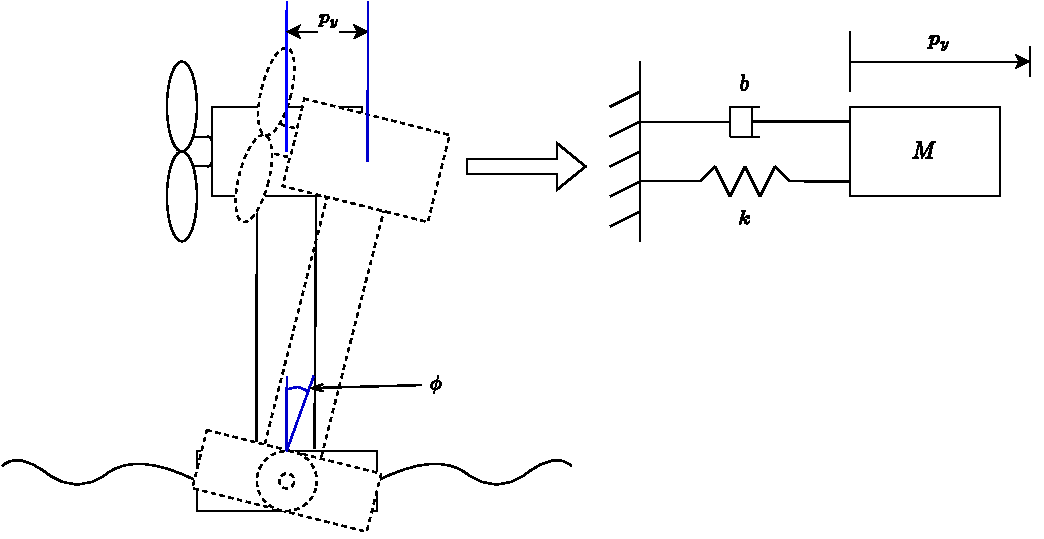
\includegraphics[width=0.9\linewidth]{../Graphics/wtLinForeAftMotionModel.pdf}
		\label{fig:wtLin_fore-aft_diagram}
	\end{figure}
\end{frame}

%%%%%%%%%%%%%%%%

\begin{frame}{Modelling}{Pitch system and FLC}
	\textbf{Pitch system}:
	\begin{equation}\label{eq:comp_pitch_freq}
		\theta = \theta_{ref}
	\end{equation}
	\textbf{FLC}:
	\begin{figure}[ht]
		\centering
		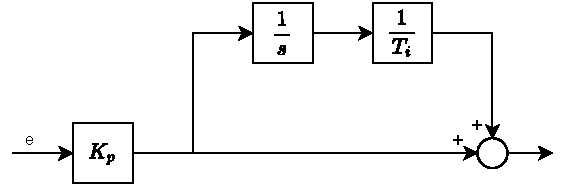
\includegraphics[width=0.65\linewidth]{../Graphics/PiController.pdf}
		\label{fig:PIcontroller}
	\end{figure}
	\begin{equation}\label{eq:comp_flc_time}
		\dot{\theta}_{ref} = K_{gs,dP/d\theta} (K_{p, \theta} \dot{e} + K_{p, \theta} \dfrac{1}{T_{i, \theta}} e)
	\end{equation}

\end{frame}

%%%%%%%%%%%%%%%%

\begin{frame}{Modelling}{Fore-aft model fitting}
	\begin{itemize}
		\item VTS allows inducing a sine on rotor speed reference and pitch angle reference
	\end{itemize}
	Fore-aft motion model parameter fitting results:
	\begin{columns}
		\begin{column}{.49\textwidth}
			\begin{figure}[ht]
				\centering
				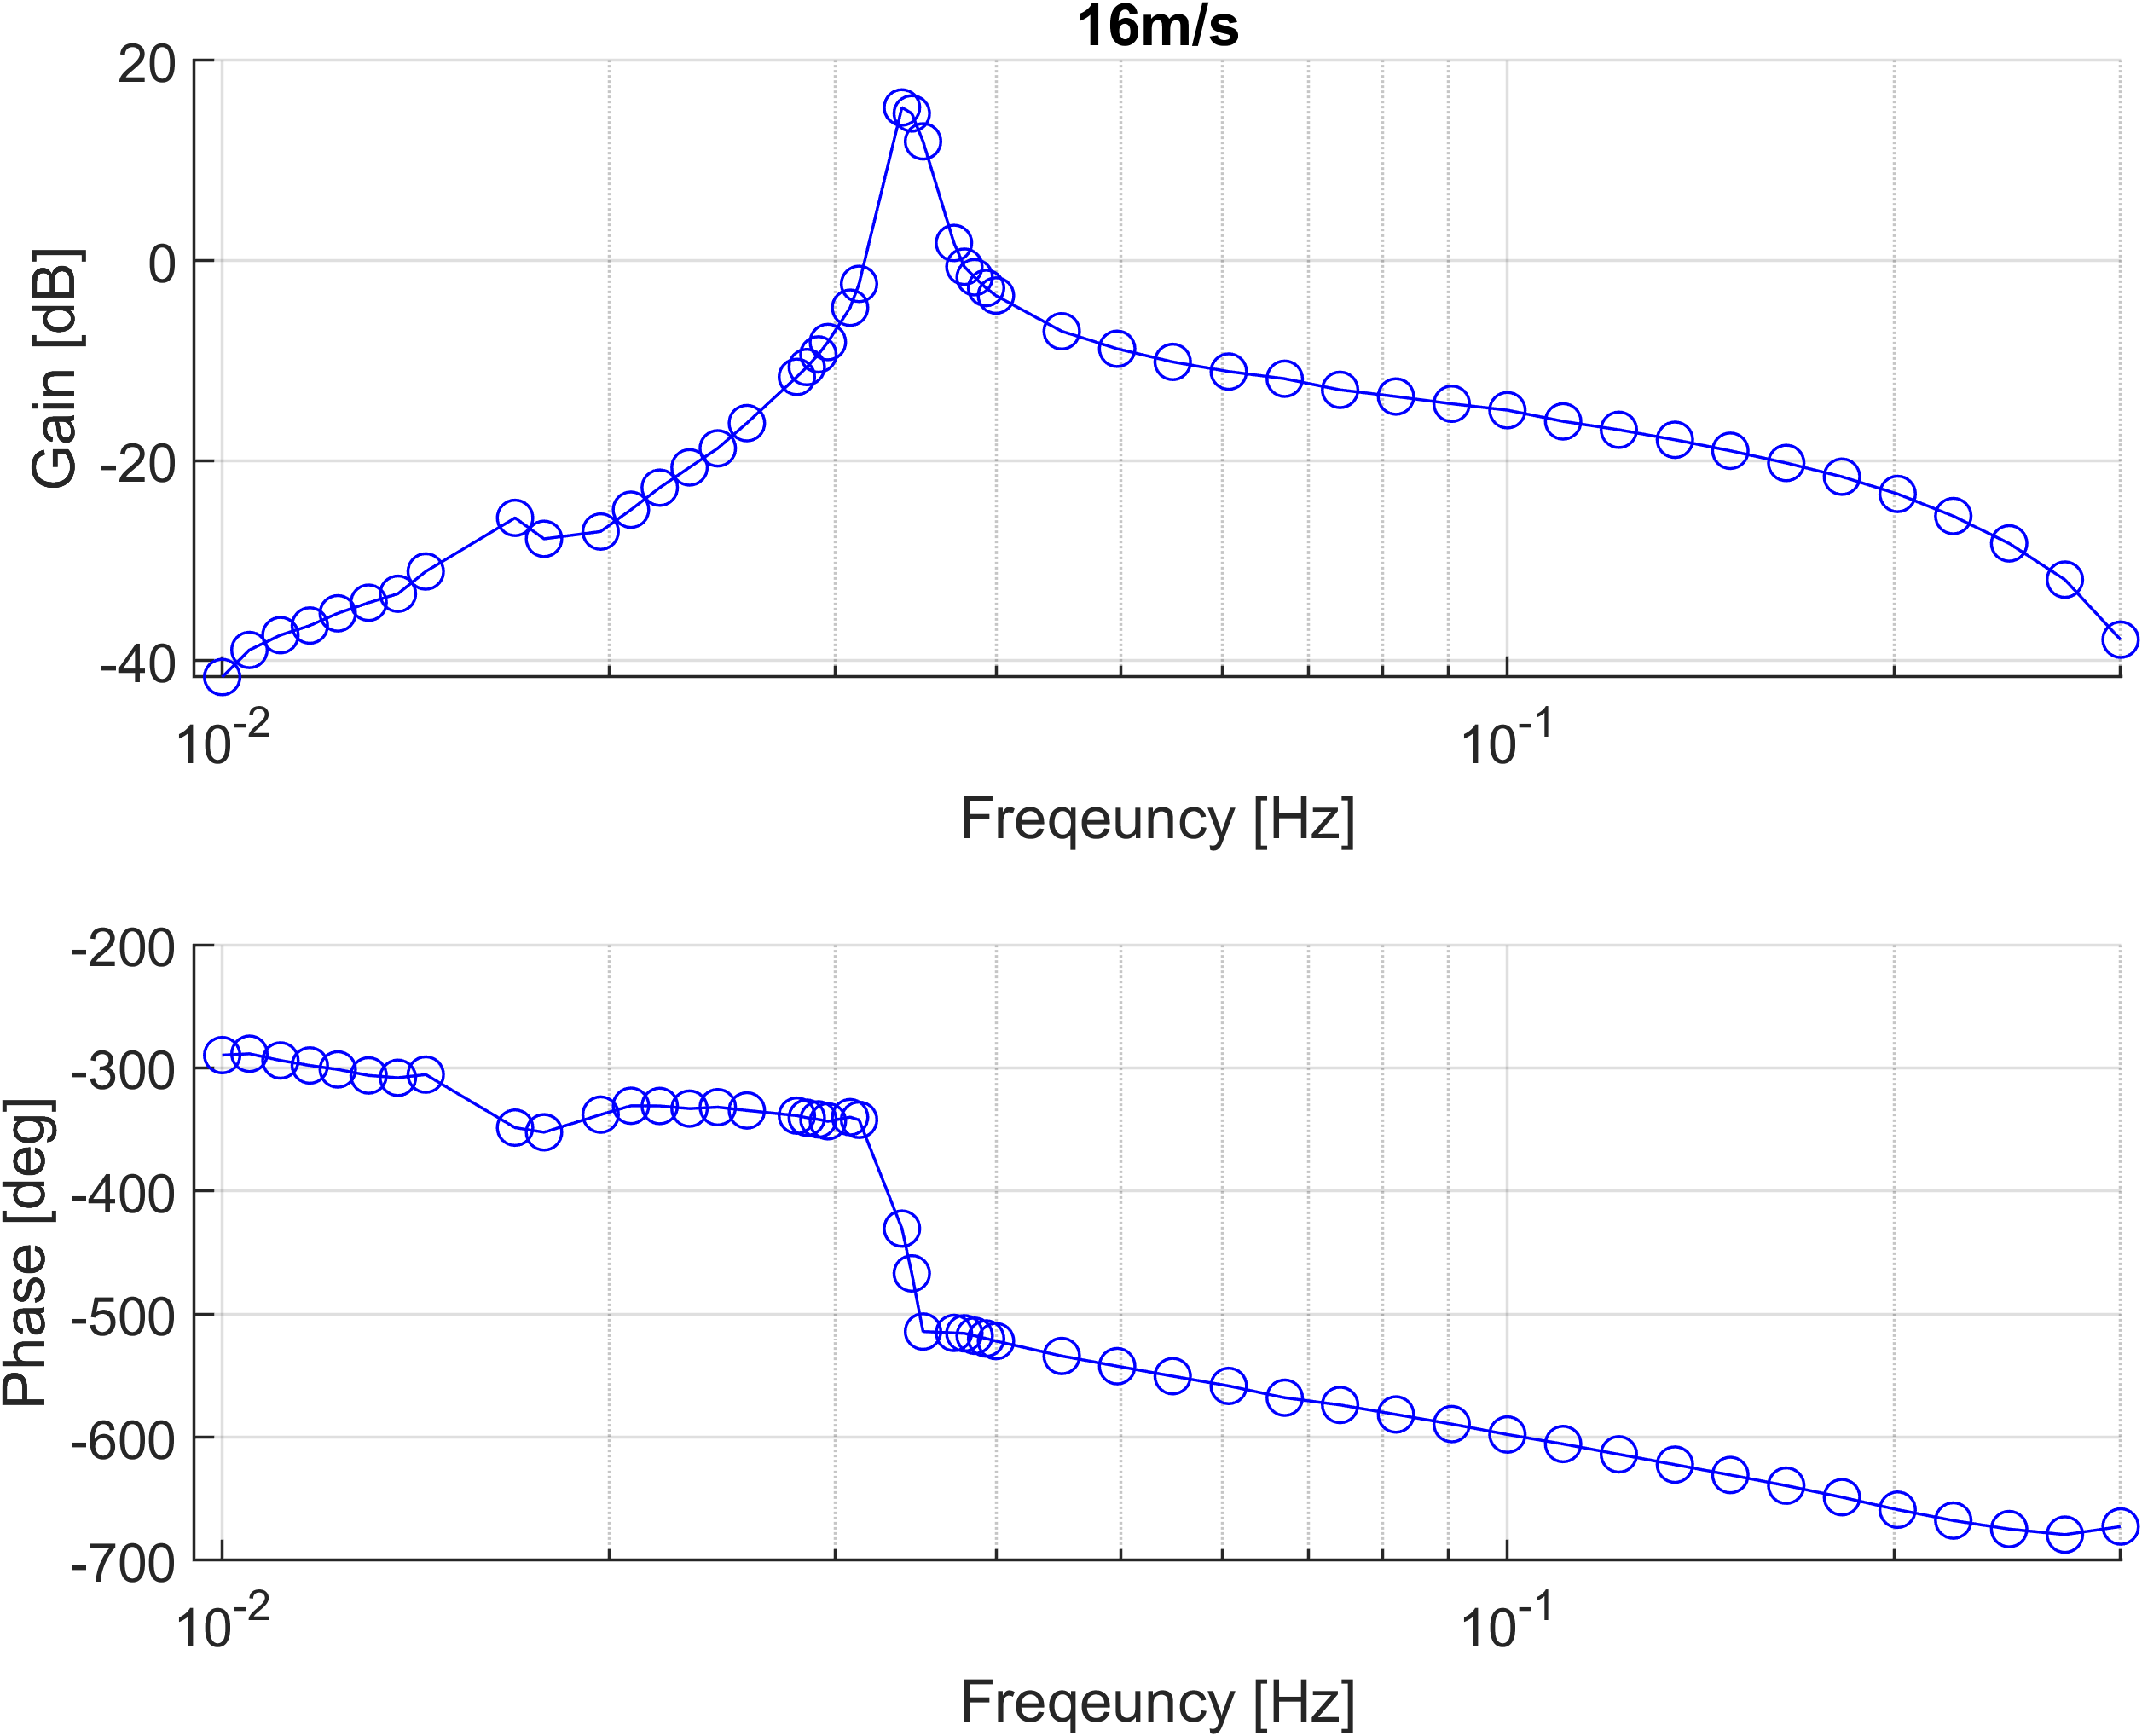
\includegraphics[width=1\linewidth]{../Graphics/TestResults/foreaftFitting/sysid_thSine-vy_16ms.png}
				\label{fig:sysid_wref-vy_16}
			\end{figure}
		\centering VTS
		\end{column}
	
		\begin{column}{.49\textwidth}
			\begin{figure}[ht]
				\centering
				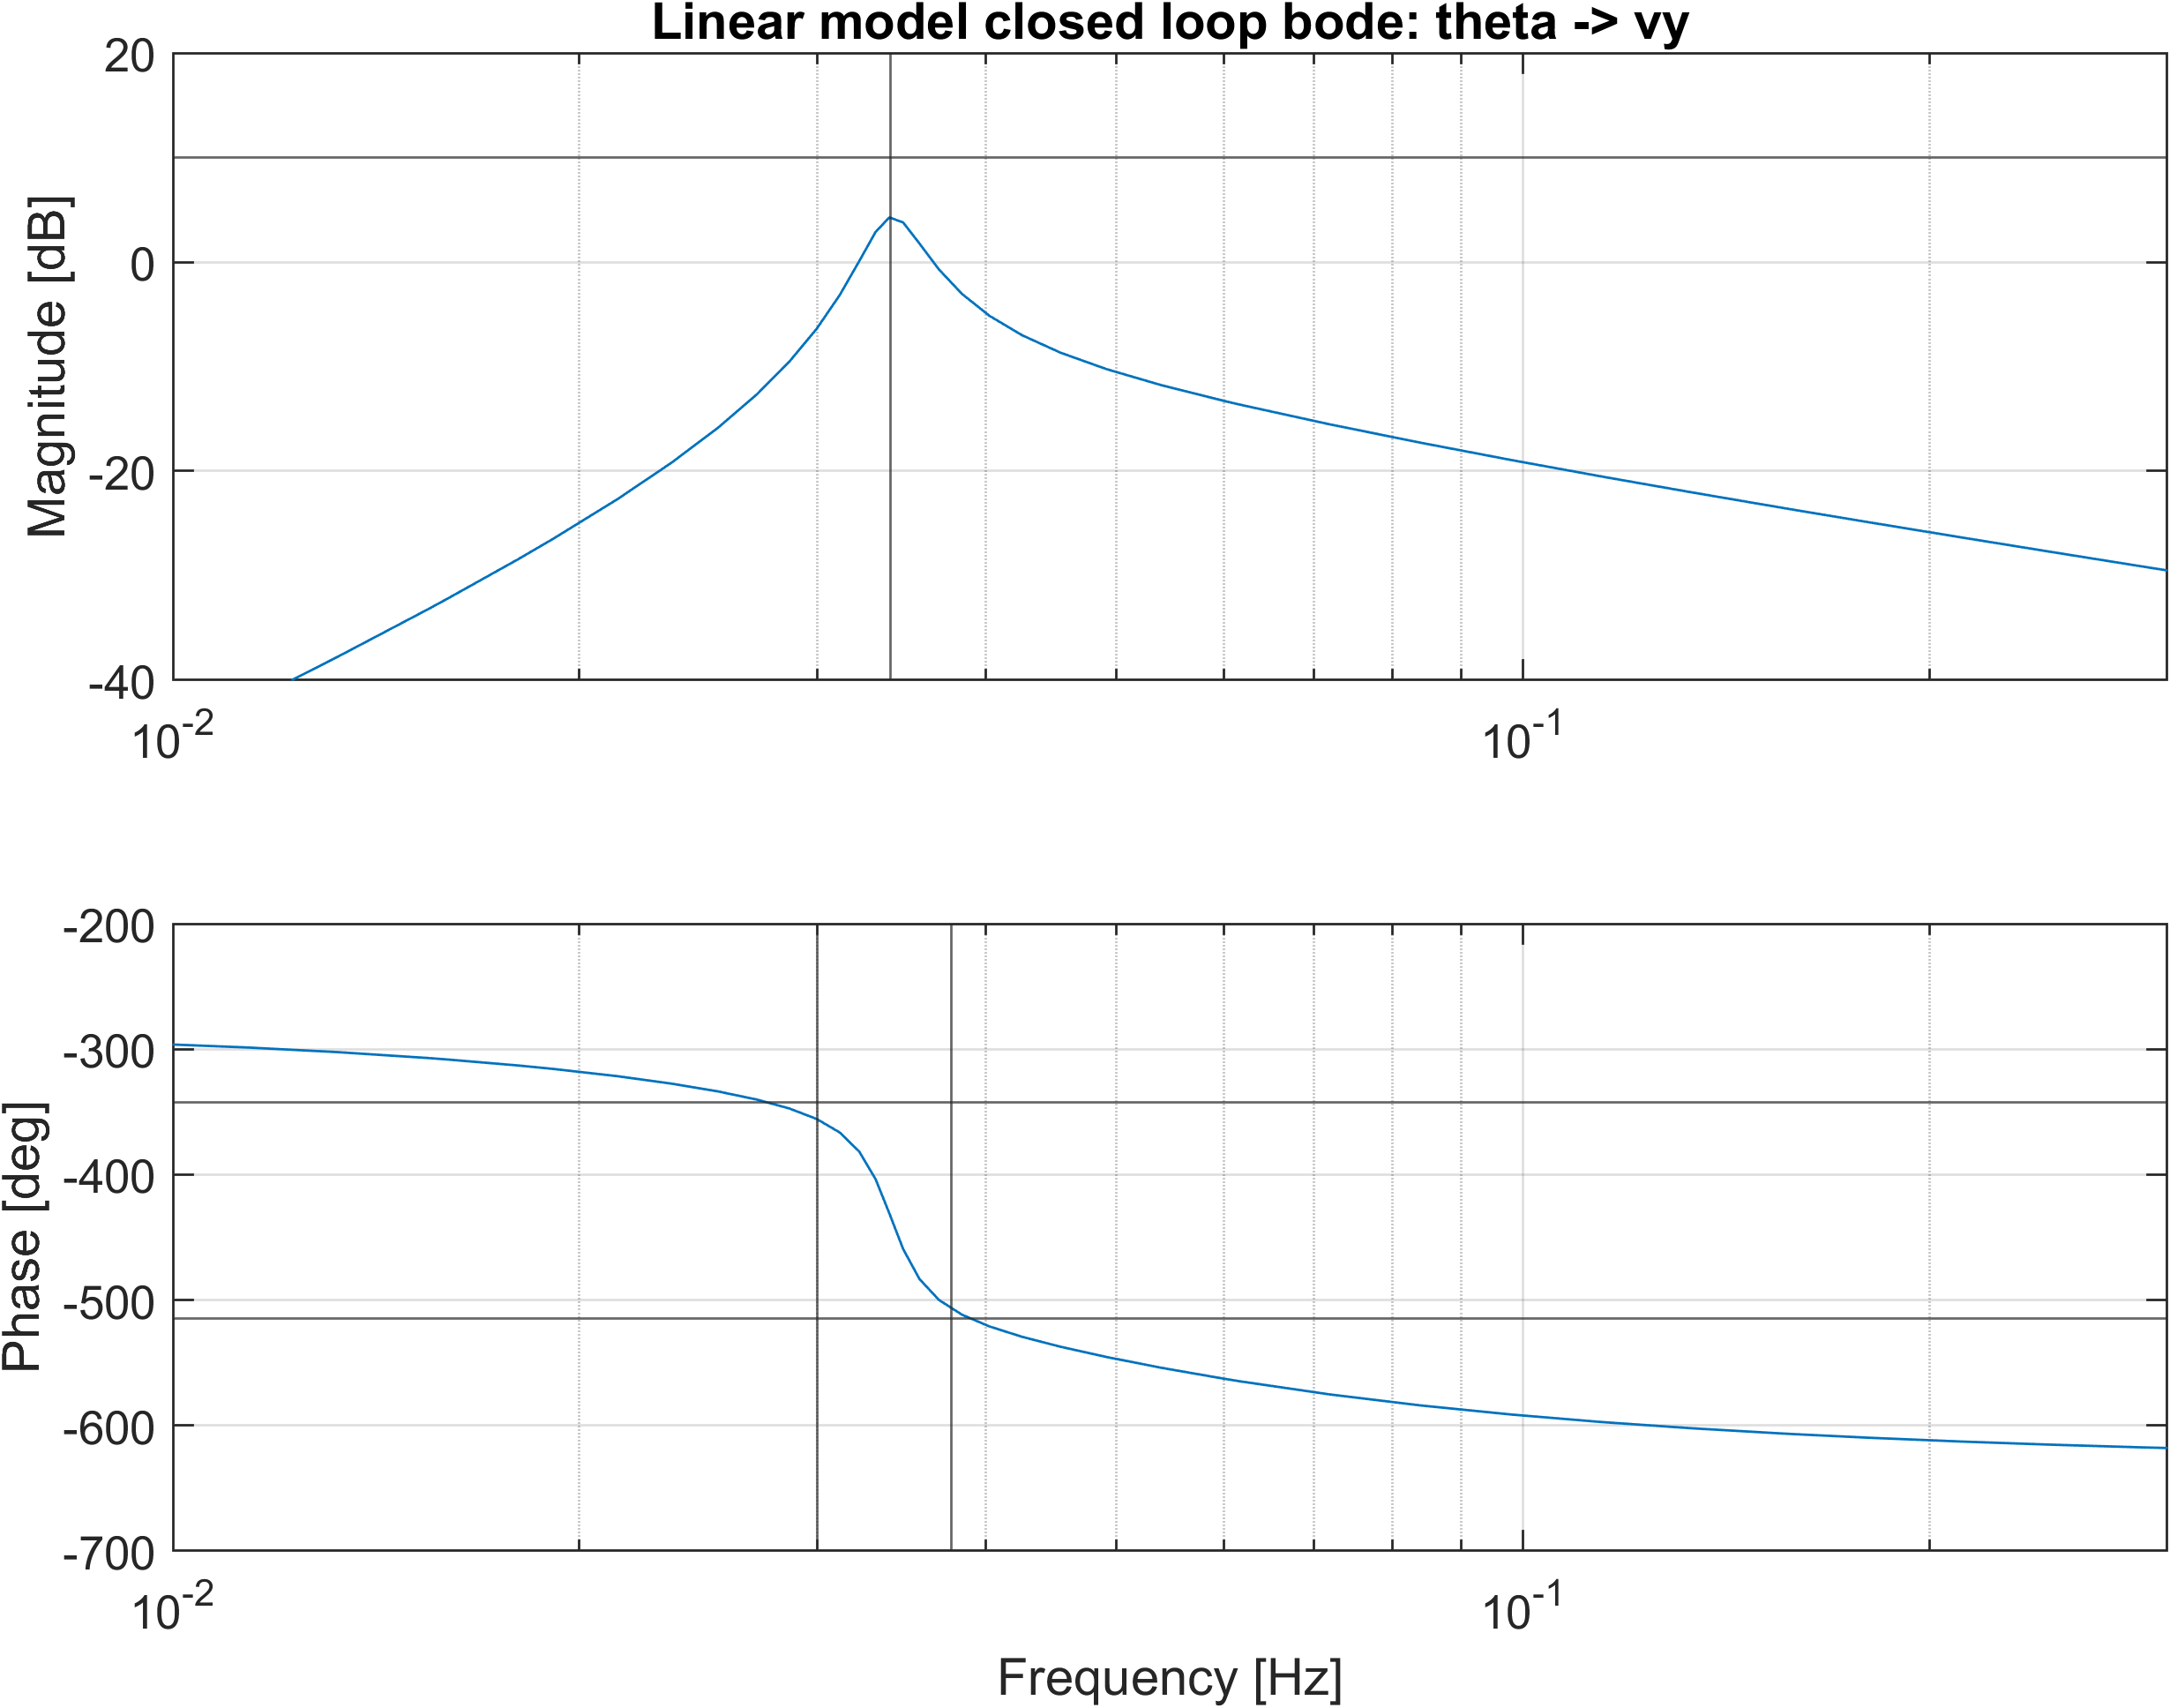
\includegraphics[width=1\linewidth]{../Graphics/TestResults/foreaftFitting/wtLin_th-vy_16ms.png}
				\label{fig:wtlin_wref-vy_16}
			\end{figure}
		\centering Linear model
		\end{column}
		
	\end{columns}
	
\end{frame}

%%%%%%%%%%%%%%%%

\begin{frame}{Modelling}{The model}
	The resulting model:
	
	\begin{itemize}
		\item \textbf{States:} \{$ p_y, v_y, \Omega, \Omega_{int} $\}
		\item \textbf{Input:} \{$ \omega_{ref} $\}
		\item \textbf{Disturbance:} \{$ v_{free} $\}
		\item \textbf{Outputs:} \{$ p_y, v_y, \Omega $\}
	\end{itemize}

	Stable
	
	\smallskip
	Controllable and observable
	
\end{frame}